\documentclass[openany]{book}
\usepackage[utf8]{inputenc}
\title{Probability Notes}
\author{Ty Darnell}
\date{ }
\usepackage[english]{babel}
 \usepackage{graphicx}
 \usepackage{float}
 \graphicspath{ {} }
 \usepackage{mathtools}
 \usepackage{amsmath, amsthm, amssymb, amsfonts}
 \usepackage{caption}
 \usepackage{titlepic}
\usepackage{hyperref}
\hypersetup{
    colorlinks=true,
    linkcolor=blue,
    filecolor=magenta,      
    urlcolor=cyan,
    pdftitle={Probability Notes},
    pdfauthor={Ty Darnell},
    bookmarksopen=true,
}
\numberwithin{equation}{section}
\newtheorem{proposition}{Proposition}[section]
\begin{document}
\titlepic{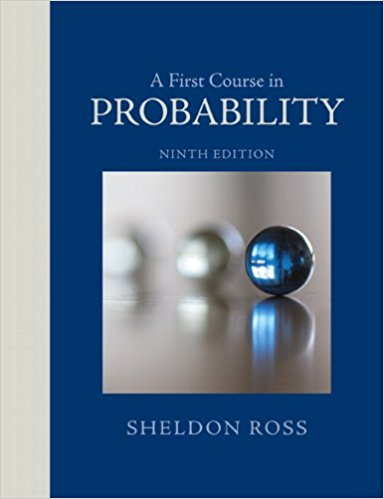
\includegraphics[scale=.8]{prob.png}}
\maketitle
\tableofcontents
\begin{flushleft}
\chapter{Combinatorial Analysis}
\section{Introduction}
The math theory of counting is known as \textbf{combinatorial analysis}	
\section{The Basic Principle of Counting}
There are $n_1 \cdot n_2 \cdots n_r$ possible outcomes of the $r$ experiments
\section{Permutations}
\[ \frac{n!}{n_1! \, n_2! \cdots n_r! }
\]
\textbf{Permutation with Replacement}: $n^r$
\section{Combinations}
\[ {n\choose r}=\frac{n!}{(n-r)! \, r!}
\]
\textbf{Combination with Replacement}:
\[\binom{r+n-1}{r}
\]
\textbf{A useful combinatorial identity}:
\[ {n\choose r}= {n-1 \choose r-1} + {n-1 \choose r} \quad 1\leq r \leq n
\]
\subsection{The Binomial Theorem}	
\[ (x+y)^n=\sum_{k=0}^{n}{n\choose k} x^k y^{n-k}
\]
\section{Multinomial Coefficients}	
A set of $n$ distinct items is to be divided into $r$ distinct groups of respective sizes $n_1,n_2,\dots,n_r$ where $\sum_{i=1}^{r}n_i = n$
\[{n\choose n_1,n_2,\dots,n_r} = \frac{n!}{n_1!\, n_2! \cdots n_r!}
\]
The numbers ${n\choose n_1,n_2,\dots,n_r}$ are known as \textbf{multinomial coefficients}
\subsection{The Multinomial Theorem}
\[(x_1+x_2+\cdots+x_r)^n = \sum_{n_1 + \cdots + n_r =n} {n\choose n_1,n_2,\dots,n_r} x_1^{n_1}x_2^{n_2}\cdots x_r^{n_r}
\]
That is, the sum is over all nonnegative integer-valued vectors $(n_1,n_2,\dots,n_r)$ such that $n_1 + n_2 + \cdots + n_r =n$
\section{The Number of Integer Solutions of Equations}
There are $r^n$ possible outcomes when $n$ distinguishable balls are to be distributed into $r$ distinguishable urns. \medbreak
If the balls are indistinguishable then they outcome of the experiment can be described by a vector $(x_1,x_2,\dots,x_r)$, where $x_i$ denotes the number of balls in the $ith$ urn. \medbreak
The problem reduces to finding the number of distinct nonnegative integer-valued vectors such that \[x_1+x_2+\cdots+x_r=n\]
\textbf{Proposition 6.1}: There are $\dbinom{n-1}{r-1}$ distinct positive integer-valued vectors $(x_1,x_2,\dots,x_r)$ satisfying the equation \[x_1+x_2+\cdots+x_r = n \ x_i>0,i=1,\dots,r\] \medbreak
\textbf{Proposition 6.2}: There are $\dbinom{n+r-1}{r-1}$ distinct nonnegative integer-valued vectors $(x_1,x_2,\dots,x_r)$ satisfying the equation \[x_1+x_2+\cdots+x_r=n\]

\chapter{Axioms of Probability}
\section{Introduction}
Concept of probability as an event, show how probabilities can be computed in certain situations
\section{Sample Space and Events}
\textbf{Sample Space}: the set of all possible outcomes of an experiment \medbreak
\textbf{Event}: Any subset of the sample space \medbreak
For any two events $E$ and $F$ of a sample space $S$, we define the new event $E \cup F$ to consist of all outcomes that are either in $E$ or in $F$ or in both. \medbreak
The event $E \cup F$ is called the \textbf{union} of $E$ and $F$ \medbreak
The event $EF$ consists of all the outcomes that are in both $E$ and $F$ and is called the \textbf{intersection} of $E$ and $F$. Also written $E \cap F$. \medbreak
$\emptyset$ is the null event, it consists of no outcomes \medbreak
If $EF = \emptyset$ then $E$ and $F$ are \textbf{mutually exclusive} since they have no outcomes in common. \medbreak
If $E_1,E_2,\dots$ are events, the union of these events, $\cup_{n=1}^{\infty}E_n$ is defined to be that event which consists of all outcomes that are in $E_n$ for at least one value of $n=1,2,\dots$ \medbreak
The intersection of the events $E_n$, $\cap^\infty_{n=1} E_n$, is the event consisting of those outcomes which are in all of the events $E_n,n=1,2,\dots$ \medbreak
$E^c$ is the \textbf{complement} of E. Consists of all outcomes in the sample space that are not in $E$ \medbreak
For any two events $E$ and $F$, if all of the outcomes in $E$ are also in $F$, then $E$ is \textbf{contained} in $F$. $E$ is a \textbf{subset} of $F$, written $E \subset F$  or equivalently $F \supset E$, meaning $F$ is a \textbf{superset} of $E$ \medbreak
If $E \subset F$ and $F \supset E$, then $E=F$ \medbreak
\textbf{Rules of Unions and Intersections}:
\begin{itemize}
\item \textbf{Commutative Laws}: $E\cup F$ = $F \cup E$ \quad $EF = FE$
\item \textbf{Associative Laws}: $(E\cup F) \cup G = E \cup (F \cup G)$ \quad $(EF)G= E(FG)$
\item \textbf{Distributive Laws}: $(E\cup F)G = EG \cup FG$ \quad $EF \cup G = (E\cup G)(F \cup G)$
\end{itemize}
\textbf{DeMorgan's Laws}:
\begin{enumerate}
\item \[ \left(\bigcup_{i=1}^n E_i\right) ^c = \bigcap_{i=1}^n E_i^c
\]
\item \[ \left( \bigcap_{i=1}^n E_i\right) ^c = \bigcup_{i=1}^n E_i^c
\]
\end{enumerate}
\section{Axioms of Probability}
\subsection{Relative Frequency Definition of Probability}
\[ P(E) = \lim_{n\to \infty} \frac{n(E)}{n}
\]
where $n(E)$ is the number of times in the first $n$ repetitions of the experiment that the event $E$ occurs \medbreak
\subsection{The Three Axioms of Probability}
\begin{enumerate}
\item $0 \leq P(E) \leq 1$
\item $P(S)=1$
\item For any sequence of mutually exclusive events $E_1,E_2,\dots$
\[ P\left(\bigcup_{i=1}^\infty E_i\right) = \sum_{i=1}^{\infty}P(E_i)
\]
\end{enumerate}
Axiom 3 states that, for any sequence of mutually exclusive events, the probability of at least one of these events occurring is just the sum of their respective probabilities.
\section{Some Simple Propositions}
\textbf{Proposition 4.1} $P(E^c)= 1-P(E)$ \medbreak
\textbf{Proposition 4.2} If $E \subset F$ then $P(E) \leq P(F)$ \medbreak
\textbf{Proposition 4.3} $P(E \cup F)= P(E) + P(F) - P(EF)$ \medbreak
\textbf{Proposition 4.4, The inclusion-exclusion identity} 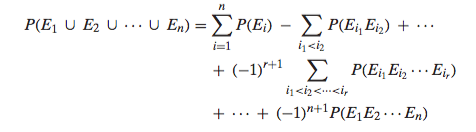
\includegraphics[scale=.6]{prop4.png}
$\sum\limits_{i_1<i_2<\cdots<i_r} P(E_{i_1}E_{i_2}\cdots,E_{i_r})$ is taken over all of the $n \choose r$ possible subsets of size $r$ of the set $\{1,2,\dots,n\}$ \medbreak
Proposition 4.4 states that the probability of the union of n events equals the sum of the probabilities of these events taken one at a time, minus the sum of the probabilities of these events taken two at a time, plus the sum of the probabilities of these events taken three at a time, and so on. \medbreak
\textbf{Inclusion-exclusion identity} can be written more succinctly: \\
$P(\cup_{i=1}^n E_i) = \sum \limits_{r=1}^{n}(-1)^{r+1} \sum \limits_{i_1<\cdots<i_r} P(E_{i_1}\cdots E_{i_r})$ 
\section{Sample Spaces Having Equally Likely Outcomes}
\[P(E)=\frac{number \, of outcomes \, in \, E}{number \, of outcomes \, in \, S}
\]
If we assume all outcomes of an experiment are equally likely to occur \medbreak
\textit{Randomly selecting k items from a set of n items}: \\
either let the outcome be the ordered selection of the k items or let it be the unordered set of items selected. \medbreak
\[ \frac{{n-1 \choose k-1}}{{n \choose k}} = \frac{k}{n}
\]
\section{Probability as a Continuous Set Function}

\section{Probability as a Measure of Belief}

\chapter{Conditional Probability and Independence}
\section{Introduction}

\section{Conditional Probabilities}
\textbf{Conditional probability} that $E$ occurs given $F$ has occurred: $P(E|F)$ \medbreak
\begin{equation}
\label{1}
P(E|F) = \frac{P(EF)}{P(F)}
\end{equation}
Multiplying both sides of \eqref{1} by $P(F)$ we get:
\begin{equation}
\label{2}
P(EF)=P(F)P(E|F)
\end{equation}
\textbf{The Multiplication Rule}:
\[P(E_1E_2E_3\cdots E_n) = P(E_1)P(E_2|E_1)P(E_3|E_1E_2)\cdots P(E_n|E_1\cdots E_{n-1})
\]
If we consider only those experiments in which $F$ occurs, then $P(E|F)$ will equal the long-run proportion of them in which $E$ also occurs.
\section{Bayes's Formula}
We can write $E$ as:
\[E=EF\cup EF^c
\]
Since all outcomes in $E$ are either in both $E$ and $F$ or in $E$ but not $F$\medbreak
Since $EF$ and $EF^c$ are clearly mutually exclusive we have:
\begin{align}
\label{3}
P(E)&=P(EF)+P(EF^c) \nonumber\\
&=P(E|F)P(F)+ P(E|F^c)P(F^c) \nonumber\\
&=P(E|F)P(F)+P(E|F^c)[1-P(F)] 
\end{align}
\textbf{Bayes Formula}
\[P(A|B)=\frac{P(B|A)P(A)}{P(B)}
\]
\textbf{Bayes' Rule with LOTP}
\begin{equation}
\label{bl}
P(A|B)=\frac{P(B|A)P(A)}{P(B|A)P(A)+P(B|A^c)P(A^c)}
\end{equation}
\subsection{Odds}
The odds of an event A tell how much more likely it is that the event A occurs
than it is that it does not occur.
\[
\frac{P(A)}{P(A^c)}=\frac{P(A)}{1-P(A)}
\]
The change in the probability of a hypothesis when new evidence is introduced can be expressed compactly in terms of the change in the odds of that hypothesis.
\begin{equation}
\label{oddsratio}\frac{P(H|E)}{P(H^c|E)}=\frac{P(H)}{P(H^c)}\frac{P(E|H)}{P(E|H^c)}
\end{equation}
The new value of the odds of $H$ is the old value, multiplied by the ratio of the conditional probability of the new evidence given that $H$ is true to the conditional probability given that $H$ is not true.
\subsection{Law of Total Probability}
\begin{equation}
\label{lotp}
P(E)=\sum_{i=1}^{n}P(E|F_i)P(F_i)
\end{equation}
\subsection{Bayes' Formula}
\begin{equation}
\label{bf}
P(F_j|E)=\frac{P(E|F_j)P(F_j)}{\sum\limits_{i=1}^{n}P(E|F_i)P(F_i)}
\end{equation}
Let $F_1,\dots, F_n$ be a set of mutually exclusive and exhaustive events (meaning that exactly one of these events must occur)\\
Suppose $E$ has occurred and we are interested in determining which one of the $F_j$ also occurred.
\section{Independent Events}
If $P(E|F)=P(E)$, $E$ is \textbf{independent} of $F$
\begin{equation}
\label{indepedence}
P(EF)=P(E)P(F)
\end{equation}
\ref{indepedence} is symmetric in $E$ and $F$
\begin{proposition}
If $E$ and $F$ are independent, then so are $E$ and $F^c$
\end{proposition}
Three events are independent if:
\begin{align*}
P(EFG)&=P(E)P(F)P(G)\\
P(EF)&=P(E)P(F)\\
P(EG)&=P(E)P(G)\\
P(FG)&=P(F)P(G)
\end{align*}
An infinite set of events is independent if every finite subset of those events is independent.
\section{$P(\cdot|F)$ is a Probability}
Conditional probabilities satisfy all of the properties of ordinary probabilities \medbreak
\textbf{Proposition 3.5.1.}
\begin{enumerate}
\item $0\leq P(E|F) \leq 1$
\item $P(S|F)=1$
\item  If $E_i,i=1,2,\dots$ are mutually exclusive events, then
\[P\bigg(\bigcup_{i=1}^{\infty}E_i|F)= \sum_{1}^{\infty}P(E_i|F \bigg)
\]
\end{enumerate}
\chapter{Random Variables}
\section{Random Variables}
Frequently, when an experiment is performed, we are interested mainly in some function of the outcome as opposed to the actual outcome itself. \medbreak
\textbf{Random Variables}: real-valued functions defined on a sample space of an experiment.\medbreak
Since the value of an r.v. is determined by the outcome of the experiment, we may assign probabilities to the possible values of the r.v.\medbreak
\textbf{Cumulative Distribution Function (CDF)}:
\[F(x)=P(X\leq x) \qquad -\infty<x<\infty
\]
\section{Discrete Random Variables}
\textbf{Probability Mass Function (PMF)} (of a discrete r.v.)
\[p(a)=P\{X=a\}
\]
$p(a)$ is the PMF of $X$
\begin{align*}
&p(x_i)\geq 0 \quad \text{for} \ i=1,2,\dots\\
&p(x) = 0 \quad \text{for all other values of} \ x
\end{align*}
\[e^x=\sum_{i=0}^{\infty}\frac{x^i}{i!}
\]
The \textbf{cumulative distribution} function $F$ can be expressed in terms of $p(a)$ by 
\[F(a)=\sum_{all \ x\leq a}p(x)
\]
If $X$ is a discrete r.v. whose possible values are $x_1,x_2,x_3,\dots$ where $x_1<x_2<x_3<\dots$ then the distribution function $F$ of $X$ is a step function.
The value of $F$ is constant in the intervals $[x_{i-1},x_i)$
and then takes a step (or jump) of size $p(x_i)$ at $x_i$.\medbreak
The size of the step at any value is equal to the
probability that $X$ assumes that particular value.
\section{Expected Value}
\textbf{Expectation} or \textbf{Expected Value} (of $X$): weighted average of the possible values that X can take on, each value being weighted by the probability that X assumes
\[E[X]=\sum_{x:p(x)>0}xp(x)
\]
where $p(x)$ is the PMF of $X$ \medbreak
If $X$ is a random variable that must take on the values $x_1,x_2,\dots,x_n$ with respective probabilities $p(x_1),p(x_2),\dots,p(x_n)$ then we have: 
\[\sum_{i=1}^{n}x_ip(x_i)=E[X]
\]
$I$ is an indicator variable for event $A$ if:
\[I=
\begin{cases}
1 & \text{if} \ A \ \text{occurs}\\
0 & \text{if} \ A^c \ \text{occurs}
\end{cases}
\]
$E[I]=P(A)$\\
The expected value of the indicator variable for the event $A$ is equal to the probability that $A$ occurs.
\section{Expectation of a Function of a Random Variable}
\begin{proposition}
If $X$ is a discrete r.v. that takes on one of the values $x_1, i\geq 1$ with respective probabilities $p(x_i)$, then for any real-valued function $g$:
\[E[g(X)]=\sum_{i}g(x_i)p(x_i)
\]
\end{proposition}
If $a$ and $b$ are constants, then
\[E[aX+b]=aE[X]+b
\]
Expected value is also called the \textbf{mean} or the \textbf{first moment of X}. \\
The quantity $E[X^n], n\geq 1$ is called the \textbf{nth moment of X}.
\[E[X^n]=\sum_{x:p(x)>0}x^np(x)
\]
\textbf{Maximizing Expected Value}: Find where the derivative equals 0
\section{Variance}
\textbf{Variance}: If $X$ is a random variable with a mean $\mu$ then:
\[Var(X)=E[(X-\mu)^2]
\]
alternatively:
\[Var(X)=E[X^2]-(E[X])^2
\]
a useful identity for any constants $a$ and $b$:
\[Var(aX+b)=a^2Var(X)
\]
\textbf{Standard Deviation}:
\[SD(X)=\sqrt{Var(X)}
\]
\section{The Bernoulli and Binomial Random Variables}
\begin{align}
\label{bern}
\begin{split}
p(0)&=P{X=0}=1-p\\
p(1)&=P{X=1}=p
\end{split}
\end{align}
\textbf{Bernoulli random variable}: An r.v. with a PMF given by \ref{bern} Has parameters $(1,p)$\medbreak

\textbf{Binomial random variable}: $n$ independent Bernoulli trials, $X$ represents number of successes and is an r.v. with parameters $(n,p)$\medbreak
The PMF of a binomial r.v.:
\begin{equation}
p(i)=\binom{n}{i}p^i(1-p)^{n-i} \qquad i=0,1,\dots,n
\end{equation}
\subsection{Properties of Binomial Random Variables}
$E[X]=np$ \medbreak
$Var(X)=np(1-p)$
\begin{proposition}
$X$ is an r.v. with parameters $(n,p)$. As $k$ goes from 0 to $n$, $P\{X=k\}$ first increases monotonically and then decreases monotonically, reaching its largest value when $k$ is the largest integer $\leq (n+1)p$.
\end{proposition}
\textbf{Stirling's Approximation} (for large $k$):
\[k!\sim k^{k+1/2}e^{-k}\sqrt{2\pi}
\]
\subsection{Computing the Binomial Distribution Function}
Distribution function given $X$ is binomial with parameters $(n,p)$.
\[P\{X\leq i\}=\sum_{k=0}^{i}\binom{n}{k}p^k(1-p)^{n-k} \qquad i=0,1,\dots,n
\]
To compute the distribution function, utilize the relationship between $P\{X=k+1\}$ and $P\{X=k\}$
\begin{equation}
\label{bind}
P(X=k+1)=\frac{p}{1-p}\frac{n-k}{k+1}P\{X=k\}
\end{equation}
\section{The Poisson Random Variable}
\textbf{Poisson r.v.}(with parameter 
\ $\lambda>0$):
\begin{equation}
\label{poi}
p(i)=P\{X=i\}=e^{-\lambda}\frac{\lambda^i}{i!} \qquad i=0,1,2,\dots
\end{equation}
The Poisson r.v. with parameter $\lambda=np$ (the expected number of successes) may be used as an approximation for a binomial r.v. when $n$ is large and $p$ is small enough so that $np$ is of moderate size.\medbreak
$Var(X)$ and $E(X)$ are both equal to $\lambda$ \medbreak
\textbf{Poisson Paradigm}: Consider $n$ events with $p_i$ equal to the probability that event $i$ occurs, $i=1,\dots,n$. If all the $p_i$ are “small” and the trials are either independent or at most “weakly dependent,” then the number of these events that occur approximately
has a Poisson distribution with mean $\sum_{i=1}^{n}p_i$. \medbreak

Basically it is not essential that all the events have the same probability of occurrence, but only that all of these probabilities be small. \medbreak

Another use of the Poisson probability distribution arises in situations where
“events” occur at certain points in time\medbreak
Assume the following:
\begin{enumerate}
\item The Probability that exactly 1 event occurs in a given interval of length $h$ is equal to $\lambda h+o(h)$ \\
$o(h)$ stands for any function $f(h)$ for which $\lim_{h\to 0}f(h)/h=0$
\item The probability that 2 or more events occur in an interval of length $h$ is equal to $o(h)$ 
\item For any integers $n,j_1,j_2,\dots,j_n$ and any set of $n$ nonoverlapping intervals, if we define $E_i$ to be the even that exactly $j_i$ of the events under consideration occur in the $ith$ of these intervals, then events $E_1,E_2,\dots,E_n$ are independent.
\end{enumerate}
Assumptions 1 and 2 state that, for small values of $h$, the probability
that exactly 1 event occurs in an interval of size $h$ equals $\lambda h$ plus something that is small compared with $h$, whereas the probability that 2 or more events occur is small
compared with $h$.\medbreak
Assumption 3 states that whatever occurs in one interval has no
(probability) effect on what will occur in other, nonoverlapping intervals.\medbreak

 \eqref{7.2} is obtained by defining the number of events occurring in any interval of length $t$ as $N(t)$ and breaking the interval into $n$ nonoverlapping subintervals, each of length $t/n$.
\begin{multline}
\label{7.2}
P\{N(t)=k\}=P\{\text{k of the n subintervals contain exactly 1 event and other n-k contain 0 events}\}\\ + P\{N(t)=k \ \text{and at least 1 subinterval contains 2 or more events}\}
\end{multline}
\[P\{N(t)=k\}=e^{-\lambda t}\frac{(\lambda t)^k}{k!} \quad k=0,1,\dots \tag{4.7.5} \label{7.5}
\]
\subsection{Computing the Poisson Distribution Function}
If $X$ is Poisson with parameter $\lambda$, then:
\[\frac{P\{X=i+1\}}{P\{X=i\}}=\frac{e^{-\lambda}\lambda^{i+1}/(i+1)!}{e^{-\lambda}\lambda^{i}/i!}=\frac{\lambda}{i+1}\tag{4.7.6} \label{7.6}
\]
We can use \eqref{7.6} to compute successively:
\begin{align*}
P\{X=1\}&=\lambda P\{X=0\}\\
P\{X=2\}&=\frac{\lambda}{2}P\{X=1\}\\
&\vdotswithin{=}\\
P\{X=i+1\} &=\frac{\lambda}{i+1}P\{X=i\}
\end{align*}

\section{Other Discrete Probability Distributions}
\subsection{The Geometric Random Variable}
Suppose that independent trials, each having a probability $p$, $0<p<1$, of being a success, are performed until a success occurs. If $X$ equals the number of trials required, then:
\begin{equation}
\label{4.8.1}
P\{X=n\}=(1-p)^{n-1}p \qquad n=1,2,\dots
\end{equation}
In order for $X=n$ the first $n-1$ trials are failures and the $nth$ trial is a success. \medbreak
Any r.v. $X$ whose PMF is given by \eqref{4.8.1} is a \textbf{geometric} r.v. with parameter $p$. \medbreak
The probability that at least $k$ trials are necessary to obtain a success is equal to the probability that the first $k-1$ trials are all failures:
\[P\{X\geq k\}=(1-p)^{k-1}
\]
Expected value of a geometric r.v.
$E[X]=\dfrac{1}{p}$ \medbreak
$Var(X)=\dfrac{1-p}{p^2}$
\subsection{The Negative Binomial Random Variable}
Suppose that independent trials, each having probability $p$, $0<p<1$, of being a
success are performed until a total of $r$ successes is accumulated. $X$ equals the number of required trials, then:
\begin{equation}
P\{X=n\}=\binom{n-1}{r-1}p^r(1-p)^{n-r} \qquad n=r,r+1,\dots \label{4.8.2}
\end{equation}
Any r.v. $X$ whose PMF is given by \eqref{4.8.2} is a negative binomial r.v. with parameters $(r,p)$ \medbreak
The geometric r.v. is just a negative binomial with parameter $(1,p)$ \medbreak
The probability of $r$ successes occuring before $m$ failures:
\[\sum_{n=r}^{r+m-1}\binom{n-1}{r-1}p^r(1-p)^{n-r}
\]
Expected value and variance of negative binomial:
\[E[X]=\frac{r}{p}
\]
\[Var(X)=\frac{r(1-p)}{p^2}
\]
\subsection{The Hypergeometric Random Variable}
Suppose that a sample of size $n$ is to be chosen randomly (without replacement) from an urn containing $N$ balls, of which $m$ are white and $N-m$ are black. $X$ is the number of white balls selected.
\[P{X=i}=\frac{\binom{m}{i}\binom{N-m}{n-i}}{\binom{N}{n}} \quad i=0,1,\dots,n \tag{4.8.4} \label{4.8.4}
\]
An r.v. $X$ whose PMF is given by \eqref{4.8.4} for some values of $n,N,M$ is a hypergeometric r.v.\medbreak

\textbf{Maximum Likelihood Estimate}: Parameter values are found such that they maximize the likelihood that the process described by the model produced the data that was actually observed.\medbreak
$P_i(N)$ is first increasing and then decreasing, and reaches its maximum value
at the largest integral value not exceeding $mn/i$. This value is the \textit{maximum likelihood estimate} of $N$. \medbreak
\textbf{Expected Value and Variance}
\[E[X]=\frac{nm}{N}
\]
\[Var(X)=\frac{nm}{N}[\frac{(n-1)(m-1)}{N-1}+1-\frac{nm}{N}]
\]
Let $p=m/N$ and rewrite as:
\[Var(X)=np(1-p)(1-\frac{n-1}{N-1})
\]
\subsection{The Zeta (or Zipf) Distribution}
\[P\{X=k\}=\frac{C}{k^{\alpha +1}} \qquad k=1,2,\dots
\]
for some $\alpha>0$
\[C=\left[\sum_{k=1}^{\infty}(\frac{1}{k})^{\alpha+1} \right]^{-1}
\]
\section{Expected Value of Sums of Random Variables}
The expected value of a sum of random variables is equal to the sum of their expectations.\medbreak
In sample space $S$, for an r.v. $X$, lets $X(s)$ be the value of $X$ when $s\in S$ is the outcome of the experiment. If $X$ and $Y$ are both r.v.s, then so is their sum. That is,\\
$Z=X+Y$ is an r.v. and $Z(s)=X(s)+Y(s)$\medbreak
Let $p(s)=P(\{s\})$ be the probability that $s$ is the outcome of an experiment.\\
Because we can write any event $A$ as the finite or countably infinite union of mutually exclusive events $\{s\},s\in A$ we have:
\[P(A)=\sum_{s\in A}p(s)
\]
\begin{proposition}
	\label{p4.9.1}
	\[E[X]=\sum_{s\in S}X(s)p(s)\]
\end{proposition}
For r.v.s $X_1,X_2,\dots,X_n$
\[E \left[\sum_{i=1}^{n}X_i\right]=\sum_{i=1}^{n}E[X_i]
\]
\section{Properties of the Cumulative Distribution Function}
For the distribution function $F$ of $X$, $F(b)$ denotes the probability that the r.v. $X$ takes on a value that is less than or equal to $b$.\medbreak
Properties of the CDF $F$:
\begin{enumerate}
\item $F$ is a nondecreasing function, if $a<b$, then $F(a)\leq F(b)$
\item $\displaystyle \lim_{b\to \infty}=1$
\item  $\displaystyle \lim_{b \to -\infty}F(b)=0$
\item $F$ is right continuous. For any $b$ and any decreasing sequence $b_n,n\geq 1$ that converges to $b$, $\displaystyle \lim_{n \to \infty}F(b_n)=F(b)$
\end{enumerate}
\[P\{x<X\leq b\}=F(b)-F(a) \qquad \text{for all }a<b
\]
\[P\{X<b\}=\lim_{n \to \infty} F \left(b-\frac{1}{n}\right)
\]
\chapter{Continuous Random Variables}
\section{Introduction}
$X$ is a \textbf{continuous random variable} if there exists a nonnegative function $f$, defined for all real $x \in (-\infty,\infty)$, having the property that for any set $B$ of real numbers:
\begin{equation}
\label{5.1.1}
P\{X \in B\}= \int_{B}f(x) \ dx
\end{equation}
The function $f$ is called the \textbf{probability density function} of $X$ \medbreak
\eqref{5.1.1} states that the probability that $X$ will be in $B$ can be obtained by integrating the pdf over the set $B$. Since $X$ must assume some value, $f$ must satisfy:
\[1=P\{X \in (-\infty,\infty) \}= \int_{-\infty}^{\infty}f(x) \ dx
\]
Letting $B=\left[a,b\right]$ we obtain:
\begin{equation}
\label{5.1.2}
P\{a\leq X \leq b \}= \int_{a}^{b}f(x)\ dx
\end{equation}
The probability that a c.r.v. will assume any fixed value is 0. \medbreak
\[P\{X<a\}=P\{X\leq a\}=F(a)=\int_{-\infty}^{a}f(x) \ dx
\]
The relationship between the cumulative distribution $F$ and the probability distribution $f$ is:
\[F(a)=P\{X \in \left(-\infty,a \right] \} = \int_{-\infty}^{a}f(x) \ dx
\]
Differentiate both sides yields:
\[\frac{d}{da}F(a)=f(a)
\]
The density is the derivative of the cdf. \medbreak
$f(a)$ is a measure of how likely it is that the r.v. will be near $a$.
\section{Expectation and Variance of Continuous Random Variables}
\[E[X]=\int_{-\infty}^{\infty}xf(x) \ dx
\]
\begin{proposition}
	\label{p5.2.1}
	If $X$ is a continuous r.v. with pdf $f(x)$, then for any real-valued function $g$:
	\[E[g(X)]=\int_{-\infty}^{\infty}g(x)f(x) \ dx
	\]
	
\end{proposition}
\textbf{Lemma 2.1}\\
For a nonnegative r.v. $Y$:
\[E[Y]=\int_{0}^{\infty}P\{Y>y \} \ dy
\]
\[E[aX+b]=aE[X]+b
\]
\textbf{Variance}
\[Var(X)=E[(X-u)^2]\] 
\[Var(X)=E[X^2]-(E[X])^2
\]
\section{The Uniform Random Variable}
An r.v. is said to be \textbf{uniformly} distributed over the interval $(0,1)$ if its pdf is given by:
\begin{equation}
	\label{5.3.1}
f(x)=\begin{cases}
1 & 0<x<1\\
0 & \text{otherwise}
\end{cases}
\end{equation}
The probability that $X$ is in any particular subinterval of $(0,1)$ equals the length of that subinterval \medbreak
 In general $X$ is a uniform r.v. on the interval $(\alpha, \beta)$ if the pdf of $X$ is given by:
 \begin{equation}
 	\label{5.3.2}
 	f(x)=\begin{cases}
 	\dfrac{1}{\beta - \alpha} & \text{if} \ \alpha<x<\beta\\
 	0 & \text{otherwise}
 	\end{cases}
 \end{equation}
The distribution function of a uniform r.v. on the interval $(\alpha, \beta)$ is given by:
\[F(a)= \begin{cases}
0 & a\leq \alpha\\
\dfrac{a-\alpha}{\beta- \alpha} & \alpha<a<\beta\\
1 & a\geq \beta
\end{cases}
\]
\[E[X]=\frac{\beta+ \alpha}{2}
\]
The expected value of an r.v. that is uniformly distributed over some interval is equal to the midpoint of that interval. \medbreak
\[Var(X)=\frac{(\beta-\alpha)^2}{12}
\]
The variance is the square of the length of the interval divided by 12.
\section{Normal Random Variables}
We say that $X$ is a \textbf{normal random variable} or $X$ is \textbf{normally distributed} with parameters $\mu$ and $\sigma^2$ if the density of $X$ is given by:
\[f(x)=\frac{1}{\sqrt{2\pi}\sigma}e^{-(x-\mu)^2/2\sigma^2} \qquad -\infty<x<\infty
\]
The density function is a bell-shaped curve that is symmetric about $\mu$. \medbreak
If $X$ is normally distributed with parameters $\mu$ and $\sigma^2$, then $Z=(X-\mu)/\sigma$ is normally distributed with parameters 0 and 1.\\
Such an r.v. is said to be a \textbf{standard,} or a \textbf{unit}, normal variable.\medbreak
\[E[X]= \mu
\]
\[Var(X)=\sigma^2
\]
The cdf of a standard normal r.v. is denoted by $\Phi(x)$:
\[\Phi(x)=\frac{1}{\sqrt{2\pi}}\int_{-\infty}^{x}e^{-y^2/2} \ dy
\]
\pagebreak
\medbreak
Use the table to get nonnegative values of $\Phi(x)$
\begin{figure}[H]
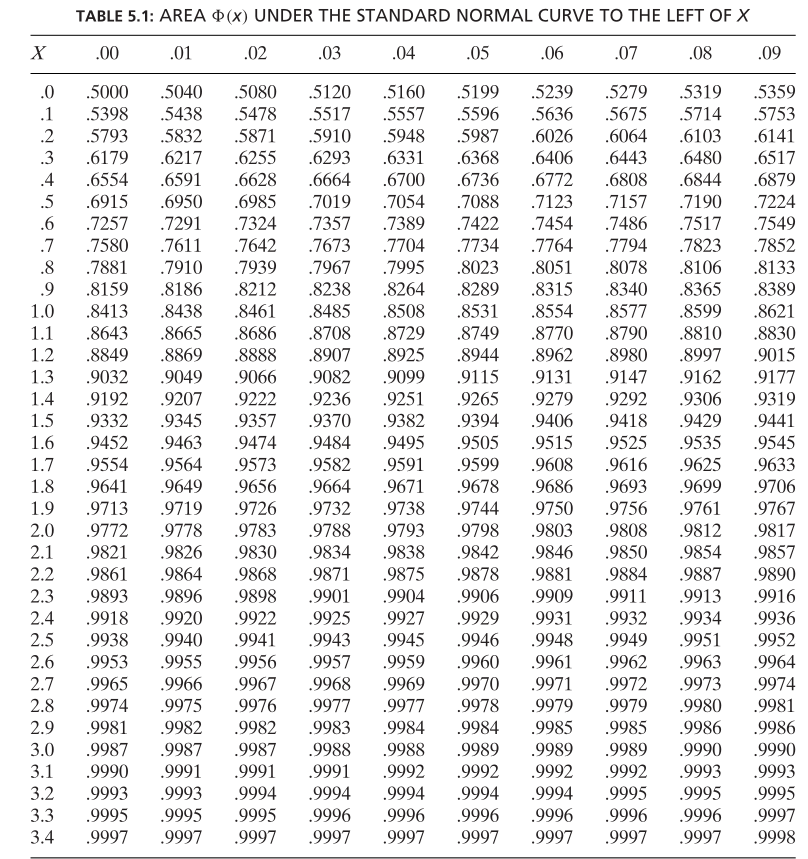
\includegraphics[scale=.8]{ncurve.png}
\end{figure}
Negative values of x, $\Phi(x)$ can be obtained from the relationship:
\begin{equation}
\label{5.4.1}
\Phi(-x)=1-\Phi(x) \qquad -\infty<x<\infty
\end{equation} 
\eqref{5.4.1} states that if $Z$ is a standard normal r.v. then:
\[P\{Z \leq -x\}=P\{Z>x\} \qquad -\infty<x<\infty
\]
Since $Z=(X-\mu)/\sigma$ is a standard normal r.v. whenever $X$ is normally distributed with parameters $\mu$ and $\sigma^2$, it follows that the distribution function of $X$ can be expressed as:
\[F_X(a)=P\{X\leq a \}=P \left(\frac{X-\mu}{\sigma}\leq \frac{a-\mu}{\sigma}\right)=\Phi \left(\frac{a-\mu}{\sigma}\right)
\]
\subsection{The Normal Approximation to the Binomial Distribution}
The \textbf{DeMoivre-Laplace limit theorem} states that when $n$ is large, a binomial r.v. with parameters $n$ and $p$ will have approximately the same distribution as a normal r.v. with the same mean and variance as the binomial. \medbreak
If we "standardize" the binomial by first subtracting its mean $np$ and then dividing the result by its standard deviation $\sqrt{np(1-p)}$, then the distribution function of this standardized r.v. (which has mean 0 and variance 1) will converge to the standard normal distribution function as $n \to \infty$\medbreak

\textbf{The DeMoivre-Laplace limit theorem}\\
If $S_n$ denotes the number of successes that occur when $n$ independent trials, each resulting in a success with probability $p$, are preformed, then, for any $a<b$:
\[P\left\{a\leq \frac{S_n-np}{\sqrt{np(1-p)}}\leq b \right\} 
\to \Phi(b)-\Phi(a)
\]
as $n \to \infty$\medbreak
The normal approximation will, in general, be good for values of $n$ satisfying $np(1-p)\geq 10$ \medbreak
\textbf{Continuity Correction}\\
Since the binomial is discrete and the normal is continuous, in order to use the normal approximation you must:
\[\text{write} \ P\{X=i\} \ \text{as} \ P\{i-1/2<X<i+1/2\}\]
\section{Exponential Random Variables}
\textbf{Exponential random variable}: with parameter $\lambda$ whose probability density function for some $\lambda>0$ is:
\[f(x)= \begin{cases} \lambda e^{-\lambda x} & \text{if} \ x\geq 0\\
0 & \text{if} \ x<0
\end{cases}
\]
The cumulative distribution function $F(a)$ of an exponential r.v. is:
\begin{align*}
F(a)&= P\{X\leq a \} \\
&= \int_{0}^{a}\lambda e^{-\lambda x} \ dx \\
&= -e^{-\lambda x} \big|_0^a\\
&= 1-e^{-\lambda a} \quad a \geq 0
\end{align*}
$E[X]=\dfrac{1}{\lambda}$\medbreak
$Var(X)=\dfrac{1}{\lambda}$\medbreak
We say that a nonnegative r.v. $X$ is \textbf{memoryless} if:
\begin{equation}
\label{5.5.1}
P\{X>s+t|X>t\}=P\{X>s\} \quad \text{for all} \ s, t\geq 0
\end{equation}
Think of $X$ as the lifetime of some instrument, \eqref{5.5.1} states that the probability that the instrument survives for at least $s+t$ hours, given that it has survived $t$ hours, is the same as the initial probability that it survives for at least $s$ hours. Basically if the instrument is alive at age $t$, the distribution of the remaining amount of time that it survives is the same as the original lifetime distribution. The instrument does not "remember" that it has already been in use for a time $t$.\medbreak
\eqref{5.5.1} is equivalent to:
\[\frac{P\{X>s+t,X>t \}}{P\{X>t\}}=P\{X>s\}
\]
\begin{equation}
\label{5.5.2}
P\{X>s+t\}=P\{X>s\}P\{X>t\}
\end{equation}
Exponentially distributed r.v.s are memoryless.
\[g(s+t)=g(s)g(t)
\]
The only right continuous solution of this functional equation is:
\begin{equation}
\label{5.5.3}
g(x)=e^{-\lambda x}
\end{equation}
Since a distribution function is always right continuous, we have:
\[\overline{F}(x)=e^{-\lambda x} \quad \text{or} \quad F(X)=P\{X\leq x\} = 1-e^{-\lambda x}
\]
\textbf{Laplace distribution}: A variation of the exponential distribution in which an r.v. that is equally likely to be positive or negative and whose absolute value is exponentially distributed with parameter $\lambda, \lambda \geq 0$. \medbreak

Its density is given by:
\[f(x)=\frac{1}{2}\lambda e^{-\lambda|x|} \qquad -\infty<x<\infty
\]
Its distribution function is given by:
\begin{figure}[H]
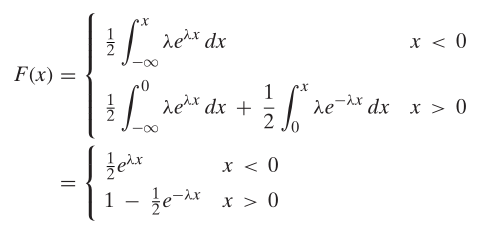
\includegraphics[scale=.7]{laplace.png}
\end{figure}
\subsection{Hazard Rate Functions}
$X$ is a positive continuous r.v. that is the lifetime of some item. Let $X$ have distribution function $F$ and density $f$.\\
The \textbf{hazard rate}(also called the \textit{failure rate}) function $\lambda(t)$ of $F$ is defined by:
\[\lambda(t)=\frac{f(t)}{\overline{F}(t)}, \quad \text{where} \ \overline{F}=1-F
\]
To interpret $\lambda(t)$, suppose that the item has survived for a time $t$ and we desire the probability that it will not survive for an additional time $dt$. That is, $P\{X \in (t, t+dt)|X>t\}$\medbreak
which  $\approx \dfrac{f(t)}{\overline{F}(t)}dt$\medbreak
Thus $\lambda(t)$ represents the conditional probability intensity that a t-unit-old item will fail.\medbreak
If the lifetime distribution is exponential, then the distribution of the remaining life for a t-year-old item is the same as that for a new item. \\
Which means $\lambda(t)=\lambda$ \medbreak
Thus the failure rate function for the exponential distribution is constant \medbreak

$\lambda$ is the rate of the distribution \medbreak
A distribution function of a positive c.r.v. can be specified by giving its hazard rate function:
\begin{equation}
\label{5.5.4}
F(t)=1-exp\left\{ -\int_{0}^{t} \lambda(t) \ dt \right\}
\end{equation}
\pagebreak
\medbreak
If an r.v. has a linear hazard rate function, that is if:\\
\[\lambda(t)=a+bt\]
Then:
\[F(t)=1-e^{-at-bt^2/2}\]
and differentiation yields its density:
\[f(t)=(a+bt)e^{-(at+bt^2/2)} \quad t\geq 0
\]
When $a=0$, the preceding equation is known as the \textit{Rayleigh density function}.
\section{Other Continuous Distributions}
\subsection{The Gamma Distribution}
An r.v. has a \textbf{gamma distribution} with parameters $(\alpha,\lambda), \ \lambda<0, \alpha >0$, if its density function is given by:
\[f(x)=\begin{cases}
\dfrac{\lambda e^{-\lambda x}(\lambda x)^{\alpha -1}}{\Gamma(\alpha)} \ &x \geq 0\\
0 \ &x<0
\end{cases}
\]
$\Gamma(\alpha)$ is the \textbf{gamma function}:
\[\Gamma(\alpha)=\int_{0}^{\infty}e^{-y}y^{\alpha-1} \ dy
\]
Integration by parts yields:
\begin{equation}
\label{5.6.1}
\Gamma(\alpha)= (\alpha-1)\Gamma(\alpha-1)
\end{equation}
For integral values of $\alpha$ say $\alpha=n$, we obtain by applying \eqref{5.6.1} repeatedly:
\[\Gamma(n)=(n-1)!
\]
When $\alpha$ is a positive integer, $\alpha=n$, the gamma distribution with parameters $(\alpha,\lambda)$ often arises as the distribution of the amount of time one has to wait until a total of $n$ evens has occurred.\medbreak
If events are occurring randomly, the amount of time one has to wait until a total of $n$ events has occurred will be a gamma r.v. with parameters $(n,\lambda)$.\medbreak
\textbf{Density function} of $T_n$ (the time its at which the $n$th even occurs):
\[f(t)=\frac{\lambda e^{-\lambda t}(\lambda t)^{n-1}}{(n-1)!}
\]
\textbf{Expected Value and Variance}:
\[E[X]=\frac{\alpha}{\lambda}
\]
\[Var(X)= \frac{\alpha}{\lambda^2}
\]
\subsection{The Weibull Distribution}
The \text{Weilbull distribution} provides a close approximation to the distribution of the lifetime
of an item, when the item dies6 when any of its parts fail.\medbreak
The Weibull distribution Function:
\begin{equation}
	\label{5.6.2}
F(x)=\begin{cases}
0 &x\leq v\\
1-exp \left\{-\left( \dfrac{x-v}{\alpha}\right)^\beta \right\} \ & x>v
\end{cases}
\end{equation}
An r.v. whose cdf is given by \eqref{5.6.2} is a \textit{Weibull r.v.} with parameters $v,\alpha,\beta$ \medbreak
Weibull Density:
\[f(x)= \begin{cases}
0 &x \leq v\\
\dfrac{\beta}{\alpha}\left(\dfrac{x-v}{\alpha} \right)^{\beta-1} exp \left\{-\left(\dfrac{x-v}{\alpha} \right)^\beta \right\} \ & x>v
\end{cases}
\]
\subsection{The Cauchy Distribution}
An r.v. has a \textbf{Cauchy distribution} with parameter $\theta , \-\infty<\theta<\infty$, if its density is given by:
\[f(x)=\frac{1}{\pi}\frac{1}{1+(x-\theta)^2} \quad -\infty<x<\infty
\]
\subsection{The Beta Distribution}
Density of a \textbf{beta distribution}:
\[f(x)=
\begin{cases}
\dfrac{1}{B(a,b)}x^{a-1}(1-x)^{b-1} \ & 0<x<1\\
0 & \text{otherwise}
\end{cases}
\]
where
\[B(a,b)=\int_{0}^{1}x^{a-1}(1-x)^{b-1} \ dx
\]
The beta distribution can be used to model a random phenomenon whose set of possible values is some finite interval $[c,d]$, which by letting $c$ denote the origin and taking $d-c$ as a unit measurement can be transformed into the interval $[0,1]$ \medbreak
When $a=b$ the beta density is symmetric about $\frac{1}{2}$, giving more and more weight to regions about $\frac{1}{2}$ as the common value $a$ increases. \medbreak
When $b>a$, the density is skewed to the left, skewed to right when $a>b$.\medbreak
The relationship
\begin{equation}
\label{5.6.3}
B(a,b)=\dfrac{\Gamma(a)\Gamma(b)}{\Gamma(a+b)}
\end{equation}
can be shown to exist between
\[B(a,b)=\int_{0}^{1}x^{a-1}(1-x)^{b-1} \ dx
\]
and the gamma function\medbreak
\textbf{Expected Value and Variance of the Beta Distribution}:
\[E[X]=\frac{a}{a+b}
\]

\[Var(X)= \frac{ab}{(a+b)^2(a+b+1)}
\]
\section{The Distribution of a Function of a Random Variable}
Suppose we know the distribution of $X$ and want to find the distribution of $g(X)$.\\
We need to express the event $g(X)\leq y$ in terms of $X$ being in some set. \medbreak
\textbf{Theorem 5.7.1}: Let $X$ be a c.r.v. having probability density function $f_X$. Suppose that $g(x)$ is a strictly monotonic differentiable (and thus continuous) function of $x$. Then the r.v. $Y$ defined by $Y=g(X)$ has a probability density function given by:
\[f_Y(y)=\begin{cases}
f_X[g^{-1}(y)] \left|\dfrac{d}{dy}g^{-1}(y) \right| & \text{if} \ y=g(x) \ \text{for some} \ x\\
0 & \text{if} \ y\neq g(x) \ \text{for all} \ x
\end{cases}
\]
where $g^{-1}(y)$ is defined to equal that value of $x$ such that $g(x)=y$.
\chapter{Jointly Distributed Random Variables}
\section{Joint Distribution Functions}
\textbf{Joint Cumulative Probability Distribution} of $X$ and $Y$:
\[F(a,b)=P\left\{X \leq a,Y \leq b \right\} \quad -\infty < a,b < \infty
\]
\textbf{Marginal Distributions} of $X$ and $Y$: \medbreak
$F_X=F(a,\infty)$ \\
$F_Y=F(\infty,b)$ \medbreak
\textbf{Joint Probability Mass Function} of $X$ and $Y$:
\[p(x,y)=P\left\{X=x,Y=y \right\}
\]
To obtain marginal pmf of $X$ or $Y$:
\begin{align*}
p_X(x) &=P\left\{X=x \right\}\\
&= \sum_{y:p(x,y)>0}p(x,y)
\end{align*}
\begin{equation*}
p_Y(y)= \sum_{x:p(x,y)>0}p(x,y)
\end{equation*}
$X$ and $Y$ are \textbf{jointly continuous} if there exists a function $f(x,y)$ defined for all real $x$ and $y$ having the property that for every set $C$ of pairs of real numbers:
\[P\left\{(X,Y) \in C \right\}=\iint\limits_{(x,y)\in C} f(x,y)  \ dx \ dy
\]
\textbf{Joint Probability Density Function}: $f(x,y)$ \medbreak
To find the joint cumulative distribution function from $f(x,y)$:\\
If $A$ and $B$ are any sets of real numbers, then by defining $C=\left\{(x,y): x\in A, y \in B \right\}$, we have:
\[P\left\{X \in A, Y \in B \right\}=\int_B \int_A f(x,y) \ dx \ dy
\]
\begin{figure}[H]
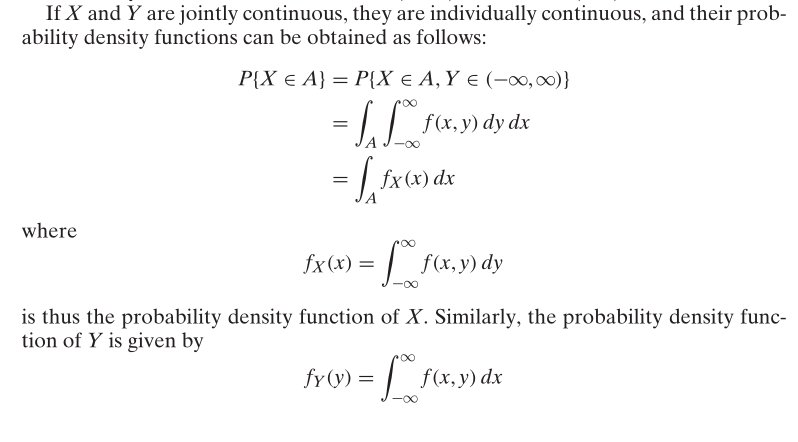
\includegraphics[scale=.7]{jointxy.png}
\end{figure}
\section{Independent Random Variables}
The r.v.s $X$ and $Y$ are \textbf{independent}, if for any two sets of real numbers $A$ and $B$:
\[P\left\{X \in A, Y \in B \right\}=P\left\{X \in A \right\} P\left\{Y \in B \right\}
\]
The above equation follows if and only if:
\[P\left\{X \leq a, Y \leq b \right\} = P\left\{X \leq a \right\} P\left\{Y \leq b \right\}
\]
In terms of the joint distribution function, $X$ and $Y$ are independent if:
\[F(a,b)=F_X(a)F_Y(b) \quad \text{for all }a,b
\]
If $X$ and $Y$ are discreet r.v.s they are independent if:
\[p(x,y)=p_X(x)p_Y(y) \quad \text{for all } x,y
\]
In the jointly continuous case, the condition of independence is equivalent to:
\[f(x,y)=f_X(x)f_Y(y) \quad \text{for all } x,y
\]
$X$ and $Y$ are independent if knowing the value of one does not change the distribution of the other. If they are not independent, they are \textbf{dependent}. \medbreak
A necessary and sufficient condition for the r.v.s $X$ and $Y$ to be independent is for their joint pdf $f(x,y)$ to factor into two terms, one depending only on $x$ and the other only on $y$.
\[f_{X,Y}(x,y)=h(x)g(y) \quad -\infty<x<\infty, -\infty<y<\infty
\]
\section{Sums of Independent Random Variables}
The cumulative distribution function $F_{X+Y}$ is called the \textbf{convolution} of the distributions $F_X$ and $F_Y$, where $X$ and $Y$ are independent.
\begin{figure}[H]
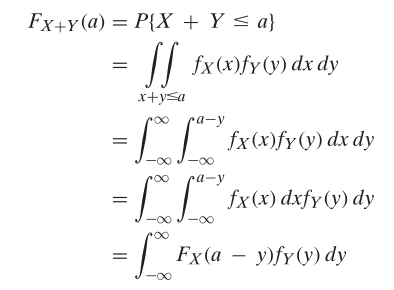
\includegraphics[scale=.7]{convo1.png}
\end{figure}
Differentiate to get the pdf $f_{X+Y}$ of $X+Y$:
\begin{align*}
\label{3.2}
\tag{3.2}
f_{X+Y}(a)&= \frac{d}{da}\int_{-\infty}^{\infty}F_X(a-y)f_Y(y)dy\\
&= \int_{-\infty}^{\infty}\frac{d}{da}F_X(a-y)f_Y(y)dy\\
&=\int_{-\infty}^{\infty}f_X(a-y)f_Y(y)dy
\end{align*}
\subsection{Identically Distributed Uniform Random Variables}
$X_1,X_2,\dots,X_n$ are independent uniform $(0,1)$ r.v.s, and:
\[F_n(x)=P\left\{X_1+\dots +X_n \leq x \right\}
\]
Then:
\[F_n(x)=x^n/{n!} \ , \quad 0 \leq x \leq 1
\]
The mean number of uniform $(0,1)$ r.v.s that must be summed for the sum to exceed 1 is equal to $e$
\subsection{Gamma Random Variables}
A gamma r.v. has a density of the form:
\[f(y)=\frac{\lambda e^{-\lambda y}(\lambda y)^{t-1}}{\Gamma(t)} \quad 0<y<\infty
\]
\textbf{Proposition 3.1}
For a fixed value of $\lambda$, the gamma distribution is closed under convolutions. \medbreak
If $X$ and $Y$ are independent gamma r.v.s with respective parameters $(s,\lambda)$ and $(t,\lambda)$, then $X+Y$ is a gamma r.v. with parameters $(s+t,\lambda)$.
\[f_{X+Y}(a)=\frac{\lambda e^{-\lambda a}(\lambda a)^{s+t-1}}{\Gamma(s+t)}
\]
\subsection{Normal Random Variables}
\textbf{Proposition 3.2} If $X_i,i=1,\dots,n$ are independent r.v.s that are normally distributed with respective parameters $\mu_i,\sigma^2_i,i=1,\dots,n$ then $\sum \limits_{i=1}^{n}X_i$ is normally distributed with parameters $\sum \limits_{i=1}^{n}\mu_i$ and $\sum \limits_{i=1}^{n}\sigma^2_i$ \medbreak

$Y$ is a \textbf{lognormal} r.v. with parameters $\mu$ and $\sigma$ if $\log(Y)$ is a normal r.v. with mean $\mu$ and variance $\sigma^2$. $Y$ is lognormal if it can be expressed as:
\[Y=e^X\]
where $X$ is a normal r.v.
\subsection{Poisson and Binomial Random Variables}
\subsection{Geometric Random Variables}
\textbf{Proposition 3.3} Let $X_1,\dots,X_n$ be independent geometric r.v.s, with $X_i$ having a parameter $p_i$ for $i=1,\dots,n$. If all the $p_i$ are distinct, then, for $k\geq n$:
\[P\left\{S_n=k \right\}=\sum_{i=1}^{n}p_iq_i^{k-1}\prod_{j \neq i}\frac{p_j}{p_j-p_i}
\]
\section{Conditional Distributions: Discrete Case}
Conditional PMF of $X$ given $Y=y$:
\begin{align*}
p_{X|Y}(x|y)&=P\left\{X=x|Y=y \right\}\\
&=\frac{P\left\{X=x,Y=y \right\}}{P\left\{Y=y \right\}}\\
&=\frac{p(x,y)}{p_Y(y)}
\end{align*}
Conditional PDF of $X$ given that $Y=y$, for all $y$ such that $p_Y(y)>0$:
\begin{align*}
F_{X|Y}(x|y)&=P\left\{X \leq x|Y=y \right\}\\
&=\sum_{a \leq x}p_{X|Y}(a|y)
\end{align*}
These are the same as the unconditional case, except that everything is now conditional on the event that $Y=y$. If $X$ is independent of $Y$, then the conditional mass function and the distribution function are the same as the unconditional ones.
\section{Conditional Distributions: Continuous Case}
Conditional probability density function of $X$ given $Y=y$, $f_Y(y)>0$:
\[f_{X|Y}(x|y)=\frac{f(x,y)}{f_Y(y)}
\]
If $X$ and $Y$ are jointly continuous, then for any set $A$:
\[P\left\{X \in A|Y=y \right\} = \int_{A}f_{X|Y}(x|y) \ dx
\]
Let $A=\left(-\infty,a\right]$, then the conditional cdf of $X$ given that $Y=y$ is:
\[F_{X|Y}(a|y)\equiv P\left\{X\leq a|Y=y \right\}=\int_{-\infty}^{a}f_{X|Y}(x|y) \ dx
\]
If $X$ and $Y$ are independent, continuous r.v.s, the conditional density of $X$ given that $Y=y$ is just the unconditional density of $X$. \medbreak
\textit{Conditional distributions when the r.v.s are neither jointly continuous nor jointly discrete}\\
If $X$ is a continuous r.v. having a pdf $f$ and $N$ is a discrete r.v., the conditional distribution of $X$ given that $N=n$ is:
\[f_{X|N}(x|n)=\frac{P\left\{N=n|X=x \right\}}{P\left\{N=n \right\}}f(x)
\]
\section{Order Statistics}
Let $X_1,X_2,\dots,X_n$ be $n$ independent and identically distributed continuous r.v.s having a common density $f$ and distribution function $F$.\\
 Define $X_{(1)}$ as the smallest, increasing with $X_{(n)}$ as the largest. \medbreak
 The ordered values $X_{(1)}\leq X_{(2)}\leq \dots \leq X_{(n)}$ are known as the \textbf{order statistics} corresponding to the r.v.s $X_1,X_2,\dots,X_n$. \medbreak
Joint density function of the order statistics:
\[f_{X(1)},\dots,X_{(n)}(x_1,x_2,\dots,x_n)=n!f(x_1)\cdots f(x_n) \quad x_1<\cdots < x_n
\]



\end{flushleft}
\end{document}